\documentclass[10pt]{extarticle}
\title{}
\author{Avinash Iyer}
\date{}
\usepackage[shortlabels]{enumitem}

%font setup
%
%\usepackage{newpxtext,eulerpx}

%paper setup
\usepackage{geometry}
\geometry{letterpaper, portrait, margin=1in}
\usepackage{fancyhdr}

%symbols
\usepackage{amsmath}
\usepackage{amsfonts}
\usepackage{mathtools}
\usepackage{hyperref}
\usepackage{gensymb}
\usepackage{multirow,array}

\usepackage[T1]{fontenc}
\usepackage[utf8]{inputenc}

%chemistry stuff
\usepackage[version=4]{mhchem}
\usepackage{chemfig}

%plotting
\usepackage{pgfplots}
\usepackage{tikz}
\tikzset{middleweight/.style={pos = 0.5, fill=white}}
\tikzset{weight/.style={pos = 0.5, fill = white}}
\tikzset{lateweight/.style={pos = 0.75, fill = white}}
\tikzset{earlyweight/.style={pos = 0.25, fill=white}}

%\usepackage{natbib}

%graphics stuff
\usepackage{graphicx}
\graphicspath{ {./images/} }

%code stuff
%when using minted, make sure to add the -shell-escape flag
%you can use lstlisting if you don't want to use minted
%\usepackage{minted}
%\usemintedstyle{pastie}
%\newminted[javacode]{java}{frame=lines,framesep=2mm,linenos=true,fontsize=\footnotesize,tabsize=3,autogobble,}
%\newminted[cppcode]{cpp}{frame=lines,framesep=2mm,linenos=true,fontsize=\footnotesize,tabsize=3,autogobble,}

\usepackage{listings}
\usepackage{color}
\definecolor{dkgreen}{rgb}{0,0.6,0}
\definecolor{gray}{rgb}{0.5,0.5,0.5}
\definecolor{mauve}{rgb}{0.58,0,0.82}

\lstset{frame=tb,
	language=Java,
	aboveskip=3mm,
	belowskip=3mm,
	showstringspaces=false,
	columns=flexible,
	basicstyle={\small\ttfamily},
	numbers=none,
	numberstyle=\tiny\color{gray},
	keywordstyle=\color{blue},
	commentstyle=\color{dkgreen},
	stringstyle=\color{mauve},
	breaklines=true,
	breakatwhitespace=true,
	tabsize=3
}
% text + color boxes
\usepackage[most]{tcolorbox}
\tcbuselibrary{breakable}
\newtcolorbox{problem}[1]{colback = white, title = {#1}, breakable}
\newtcolorbox{solution}{colback = white, colframe = black!75!white, title = Solution, breakable}
%including PDFs
\usepackage{pdfpages}
\setlength{\parindent}{0pt}

\pagestyle{fancy}
\fancyhf{}
\rhead{Avinash Iyer}
\lhead{Problem Set 1}
\begin{document}
  \begin{problem}{Gruber 2.3: Budget Constraints $+$ Choice}
    You have \$100 to spend on food ($F$) and clothing ($C$). The price of food is \$4 and the price of clothing is \$10. Assume that your utility over clothing and food is as follows:
    \[
      u(C,F) = 3\ln(C) + 7\ln(F)
    \] 
    \begin{enumerate}[(a)]
      \item Graph your budget constraint and determine the utility-maximizing choice of clothing and food.
      \item Suppose that the government subsidizes clothing such that each unit of clothing is half-price up to the first five units of clothing. Graph your budget constraint on the same figure above. What is your new utility-maximizing choice of clothing and food?
    \end{enumerate}
    \tcblower
    \begin{problem}{Graph}
      \begin{center}
        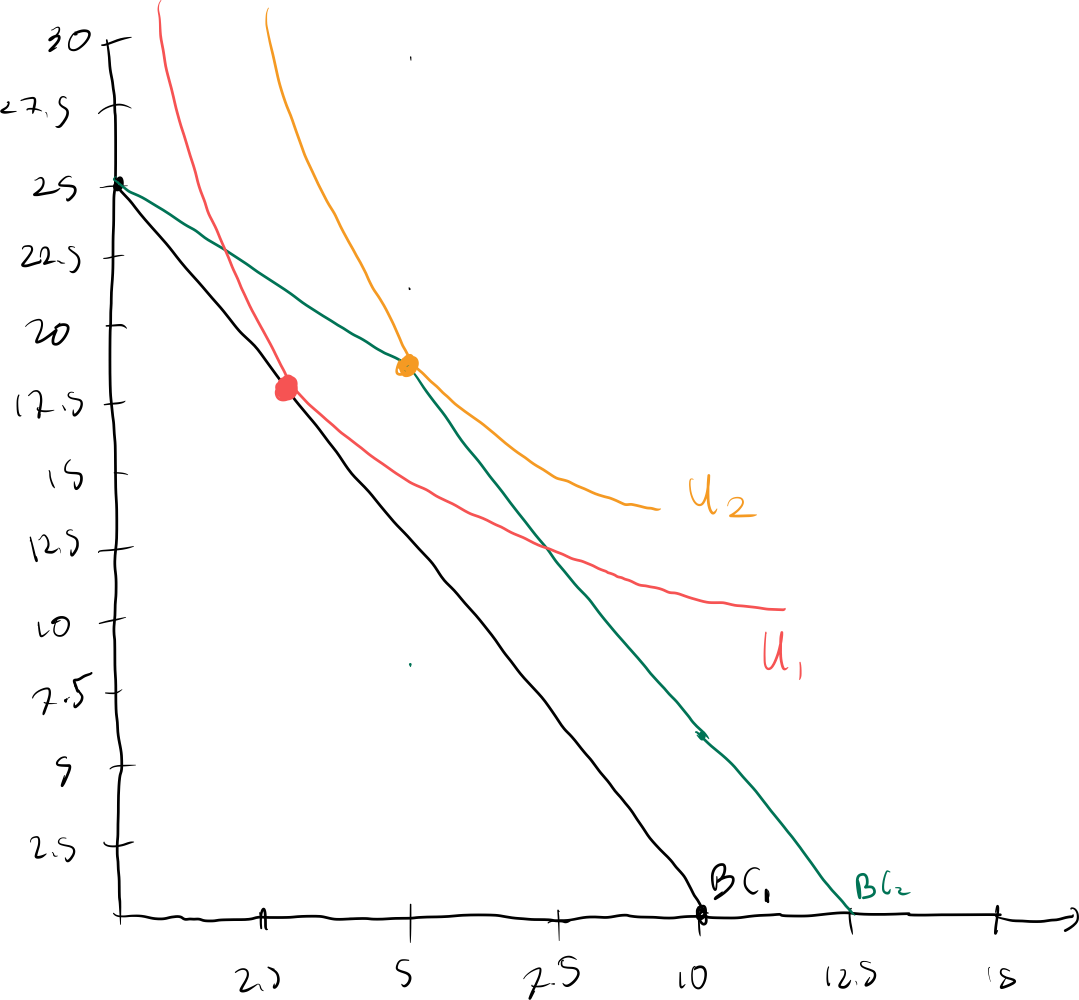
\includegraphics[width=10cm]{1_1}
      \end{center}
    \end{problem}
    \begin{problem}{(i)}
      \begin{align*}
        4F + 10C &= 100 \tag*{budget constraint}\\
        MRS_{CF} &= \frac{\frac{\partial u}{\partial C}}{\frac{\partial u}{\partial F}} \\
        \frac{10}{4}&= \frac{3F}{7C} \\
        F &= \frac{35}{6}C\\
        \frac{70}{3}C + 10C &= 100 \\
        C &= 3\\
        F &= 17.5
      \end{align*}
    \end{problem}
    \begin{problem}{(ii)}
      \begin{align*}
        \frac{16}{5}F + 8C &= 100 \tag*{component of budget constraint}\\
        MRS_{CF} &= \frac{\frac{\partial u}{\partial C}}{\frac{\partial u}{\partial F}} \\
        \frac{5}{2}&= \frac{3F}{7C} \\
        F &= \frac{35}{6}C\\
        8C + \frac{56}{3}C &= 100\\
        \frac{80}{3}C &= 100\\
        C &= 3.75\\
        F &= 18.75
      \end{align*}
      However, since the point $(3.75,18.75)$ lies outside the given component of the budget constraint, the utility maximizing point must be the kink.
    \end{problem}
  \end{problem}
  \begin{problem}{Gruber 2.13: Equity}
    The country of Adventureland has two citizens, Bill and Ted. Bill has a private legal business. He earns \$50 per hour. At a tax rate of 0\%, Bill works 20 hours per week. At a 25\% tax rate, he works only 16 hours per week, and at a 40\% tax rate he works only 8 hours per week. Ted works a manufacturing job. He works 20 hours per week and earns \$ per hour, regardless of the tax rate. The government is considering imposing an income tax of either 25\% or 40\% on Bill and using the revenues to make transfer payments to Ted. The accompanying table summarizes the three possible policies.
    \begin{center}
      \renewcommand{\arraystretch}{1.5}
      \begin{tabular}{c|c|c|c|}
        \cline{2-4}
        Rate & 0\% & 25\% & 40\% \\
        \cline{2-4}
        Bill's pretax income & \$1,000 & \$800 & \$400 \\
        \cline{2-4}
        Bill's taxes & 0 & \$200 & \$160 \\
        \cline{2-4}
        Ted's pretax income & \$120 & \$120 & \$120 \\
        \cline{2-4}
        Ted's transfer payment & 0 & \$200 & \$160\\
        \cline{2-4}
        Bill's net income & \$1000 & \$600 & \$240\\
        \cline{2-4}
        Ted's net income & \$120 & \$320 & \$280\\
        \cline{2-4}
      \end{tabular}
    \end{center}
    \begin{enumerate}[(a)]
      \item Compare the three policies. Are any of the three policies obviously less than optimal?
      \item Now suppose that Bill and Ted have the same utility function $U(Y) = Y^{1/2}$, where $Y$ is equal to net income. Rank the three tax policies discussed in part (a) for a Rawlsian social welfare function. Rank the three for a utilitarian social welfare function.
      \item How would your answer change if the utility function was $U(Y) = Y^{1/5}$?
      \item Suppose that Bill and Ted instead have different utility functions: Bill's utility is given by $U_B(Y) = 0.25Y^{1/2}$ and Ted's is given by $U_T(Y) = Y^{1/2}$. How would a Rawlsian rank the three tax policies now?
    \end{enumerate}
    \tcblower
    \begin{problem}{(a)}
      The utilities under the 40\% tax regime seem to be much lower than any of the other regimes (in terms of total net income and otherwise).
    \end{problem}
    \begin{problem}{(b)}
      \begin{center}
        \begin{tabular}{c|c|c}
          Rate & Bill's utility & Ted's utility\\
          \hline
          0\% & 31.6 & 11.0\\
          25\% & 24.5 & 17.9\\
          40\% & 15.5 & 16.7
        \end{tabular}
      \end{center}
      \begin{itemize}
        \item Rawlsian: 25\% > 40\% > 0\%
        \item Utilitarian: 0\% > 25\% > 40\%
      \end{itemize}
    \end{problem}
    \begin{problem}{(c)}
      \begin{center}
        \begin{tabular}{c|c|c}
          Rate & Bill's utility & Ted's utility\\
          \hline
          0\% & 4.0 & 2.6\\
          25\% & 3.6 & 3.2\\
          40\% & 3.0 & 3.1
        \end{tabular}
      \end{center}
      \begin{itemize}
        \item Rawlsian: 25\% > 40\% > 0\%
        \item Utilitarian: 25\% > 0\% > 40\%
      \end{itemize}
    \end{problem}
  \end{problem}
  \begin{problem}{Gruber 3.16: Drinking Health}
    More than 100 observational studies have found a link between moderate drinking and improved cardiovascular health. In these studies, moderate drinking has been shown to be associated with reduced risk of heart attack, stroke, and deaths from all cardiovascular causes. The studies find a remarkably consistent effect, with a 25\% to 40\% reduction in risk observed across an array of countries, in both men and women, and across all age groups. Suppose that you are a physician reviewing this evidence. Will you recommend to your patients who are infrequent drinkers or abstainers that they should increase their consumption of alcohol?
    \tcblower
    I would not recommend my patients to increase their consumption of alcohol --- a confounder in this data is the income level of drinkers vs. non-drinkers, as people who drink alcohol tend to be richer than those who do not drink alcohol. The differences in cardiovascular health can be potentially attributed to income --- and even if controlled for income, differences in cardiovascular health may be counteracted by negative changes in other causes of mortality.
  \end{problem}
  \begin{problem}{Gruber 3.7: Credibly Causal}
    You are hired by the government to evaluate the impact of a policy change that affects one group of individuals but not another. Suppose that before the policy change, members of a group affected by the policy averaged \$17,000 in earnings, and members of a group unaffected by the policy averaged \$16,400. After the policy change, members of the affected group averaged \$18,200 in earnings while members of the unaffected group averaged \$17,700 in earnings.
    \begin{enumerate}[(a)]
      \item Provide a credibly causal estimate of the impact of the policy change? What is the name for this type of estimation?
      \item What are the assumptions you have to make for this to be a valid estimate of the impact of the policy change?
    \end{enumerate}
    \tcblower
    \begin{problem}{(a)}
      The credibly causal estimate of the impact of the policy change is $-\$100$, which is found via difference in difference estimation (the difference between group A and group B as a result of the policy change reduced by \$100).
    \end{problem}
    \begin{problem}{(b)}
      In order for this to be a valid estimate of the impact of the policy change, we have to assume that if it were not for the policy, the income growth of group A would have been identical to that of group B.
    \end{problem}
  \end{problem}
\end{document}
